\section*{Engineering Drawings}

This appendix contains the revision-controlled technical drawings and
optional supporting material for the Helike \#213 subsystems.

\subsection{Drawing List}

The revision-controlled drawing set is listed in
Table~\ref{tab:drawings}. The electrical schematic of the subsystem
is presented in Fig.~\ref{fig:schematic}, the mechanical frame in
Fig.~\ref{fig:alba-frame} and the SRAB assembly in
Fig.~\ref{fig:srab-assembly}:

\begin{table}[htbp]
\centering
\small
\setlength{\tabcolsep}{6pt}
\begin{tabular}{>{\raggedright\arraybackslash}p{6cm}}
\toprule
\textbf{Drawing / Document} \\
\midrule
Electrical schematic (KiCad, U1--U6, SW1--SW3) \\
1P Alba Orbital frame (aluminum + FRP backplate) \\
SRAB wing assembly (hub + 2 wings, PETG) \\
SRAB wing geometry — Asa1 contour (DXF) \\
SRAB wing geometry — Asa2 contour (DXF) \\
SRAB wing geometry — Asa3 contour (DXF) \\
PocketQube 1P mechanical structure \\
ESP32-C3 pinout \\
Integrated assembly \\
\bottomrule
\end{tabular}
\caption{Drawing list.}
\label{tab:drawings}

\end{table}

\begin{figure}[htbp]
\centering
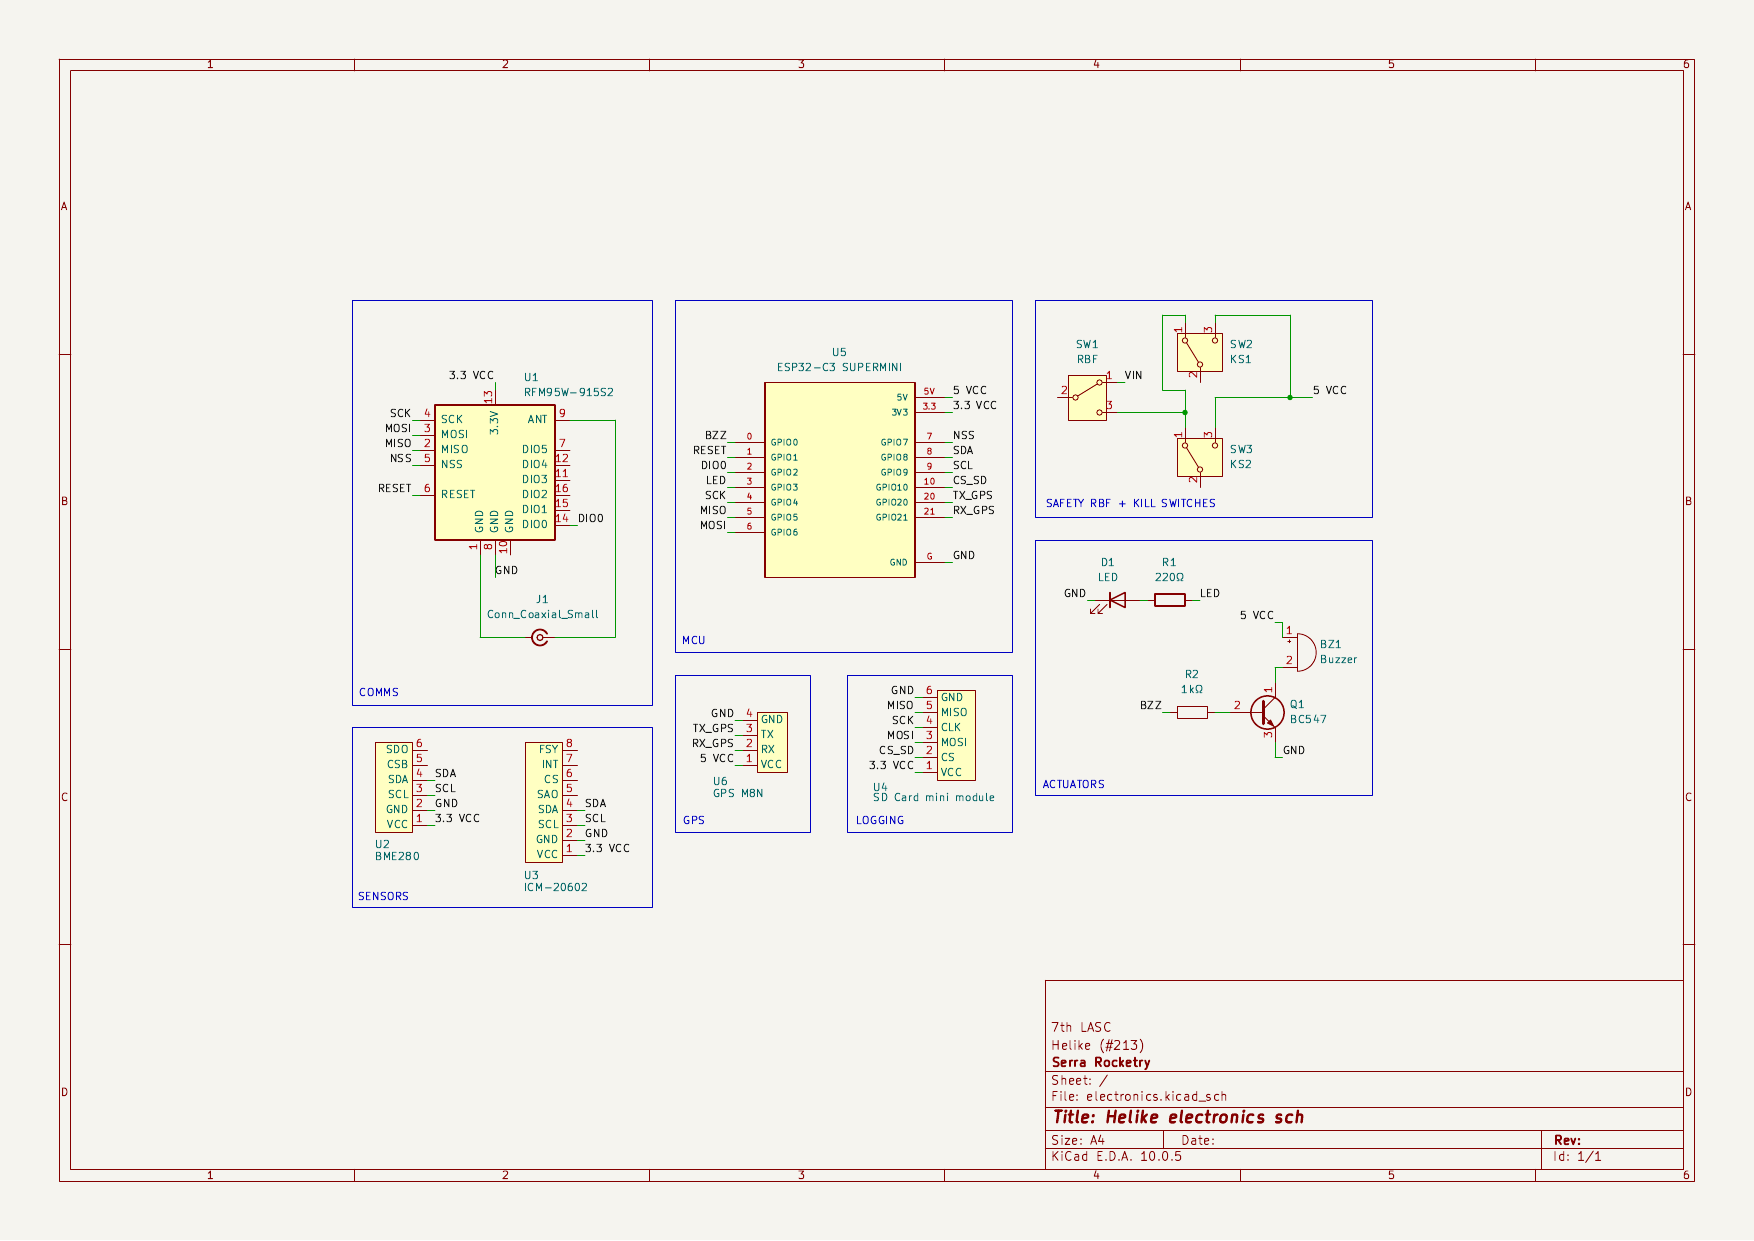
\includegraphics[width=0.9\textwidth]{figures/fig_schematic.png}
\caption{Electrical schematic of Helike \#213 (KiCad). U1: ESP32-C3
Super Mini; U2: LoRa RFM95W-915S2; U3: BME280; U4: ICM-20602; U5: GPS
NEO-8M; U6: SD card module; SW1/SW2: kill switches (Z axis); SW3: RBF
pin; J1: SMA antenna; D1/BZ1: status LED and buzzer.}
\label{fig:schematic}
\end{figure}

\begin{figure}[htbp]
\centering
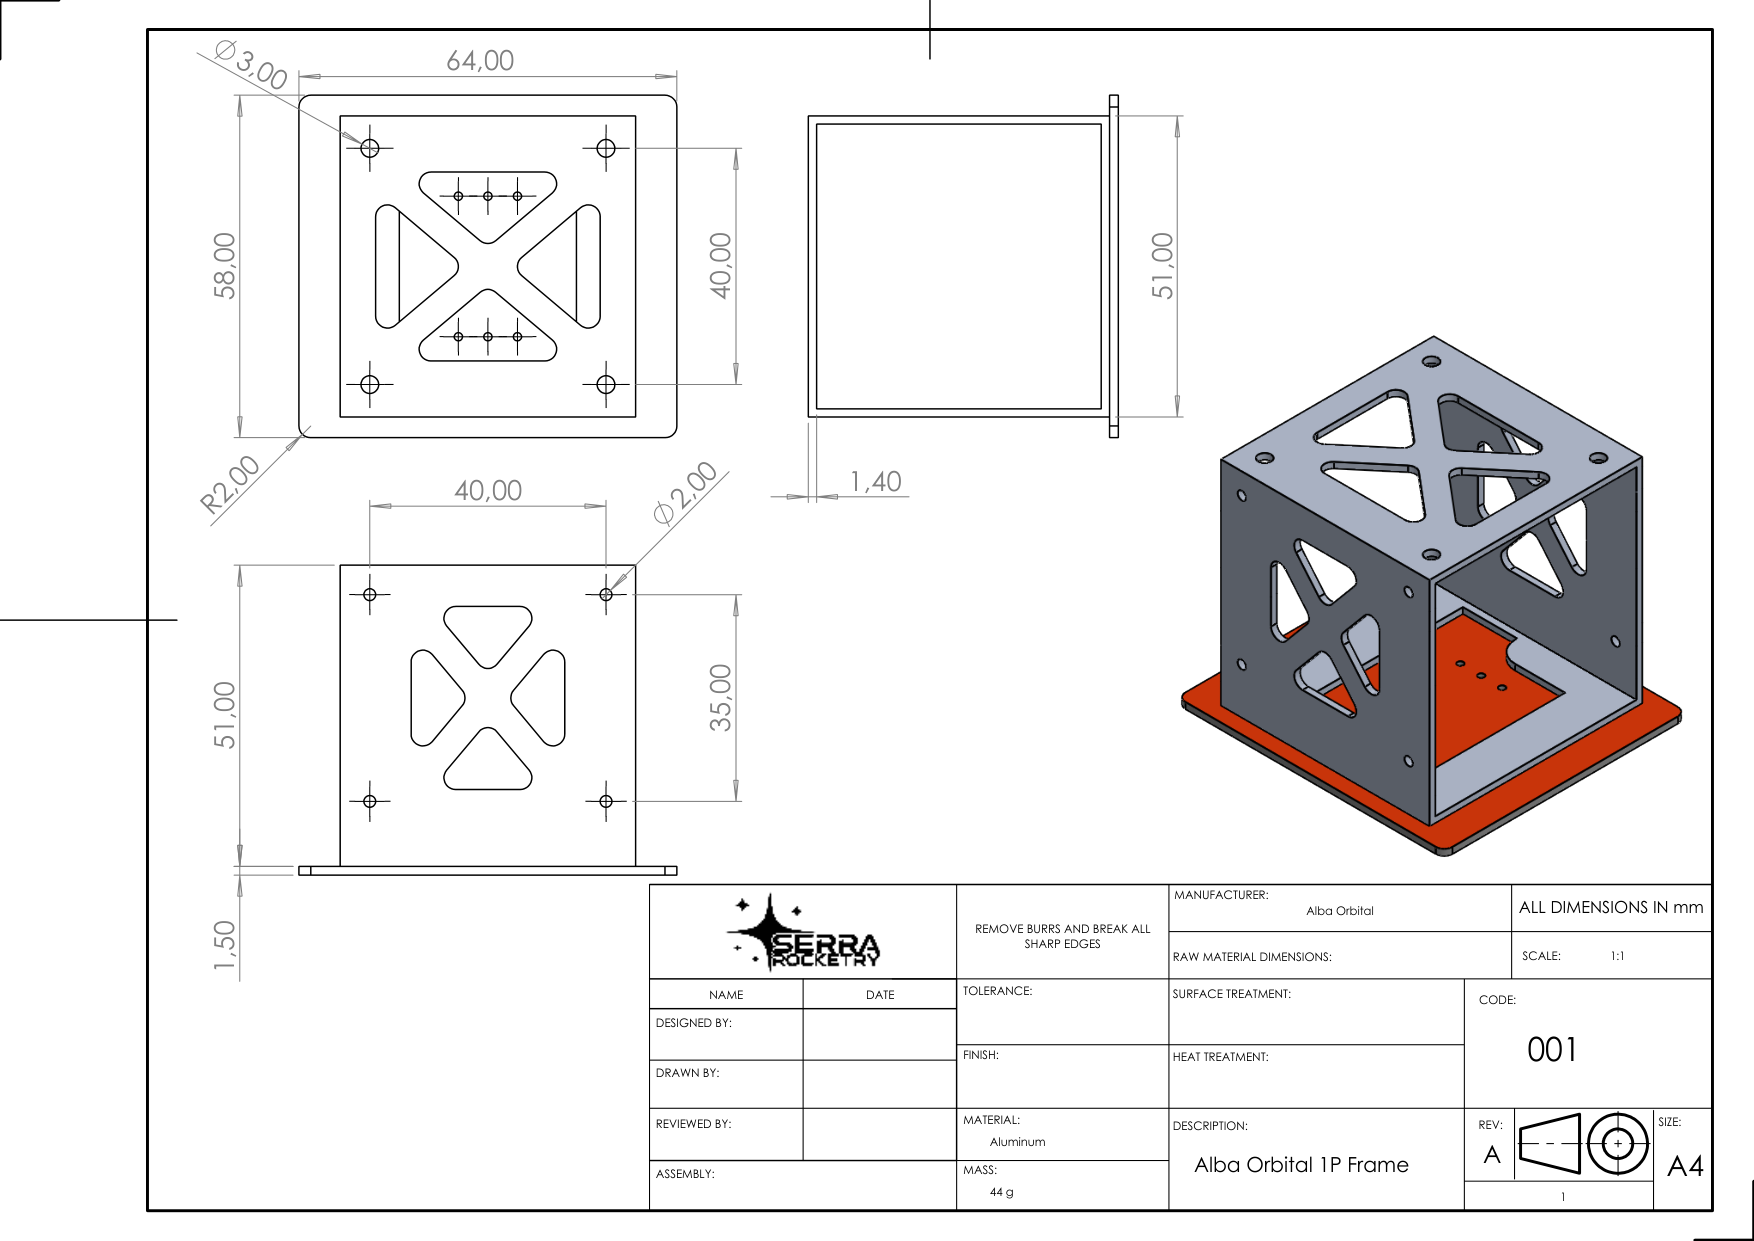
\includegraphics[width=0.8\textwidth]{figures/1P_ALBA_ORBITAL_frame_p1.png}
\caption{Technical drawing of the 1P Alba Orbital frame: 51$\times$51
mm aluminum structure with 1.4~mm wall thickness, 1.5~mm FRP
backplate and a total mass of 44~g.}
\label{fig:alba-frame}
\end{figure}

\begin{figure}[htbp]
\centering
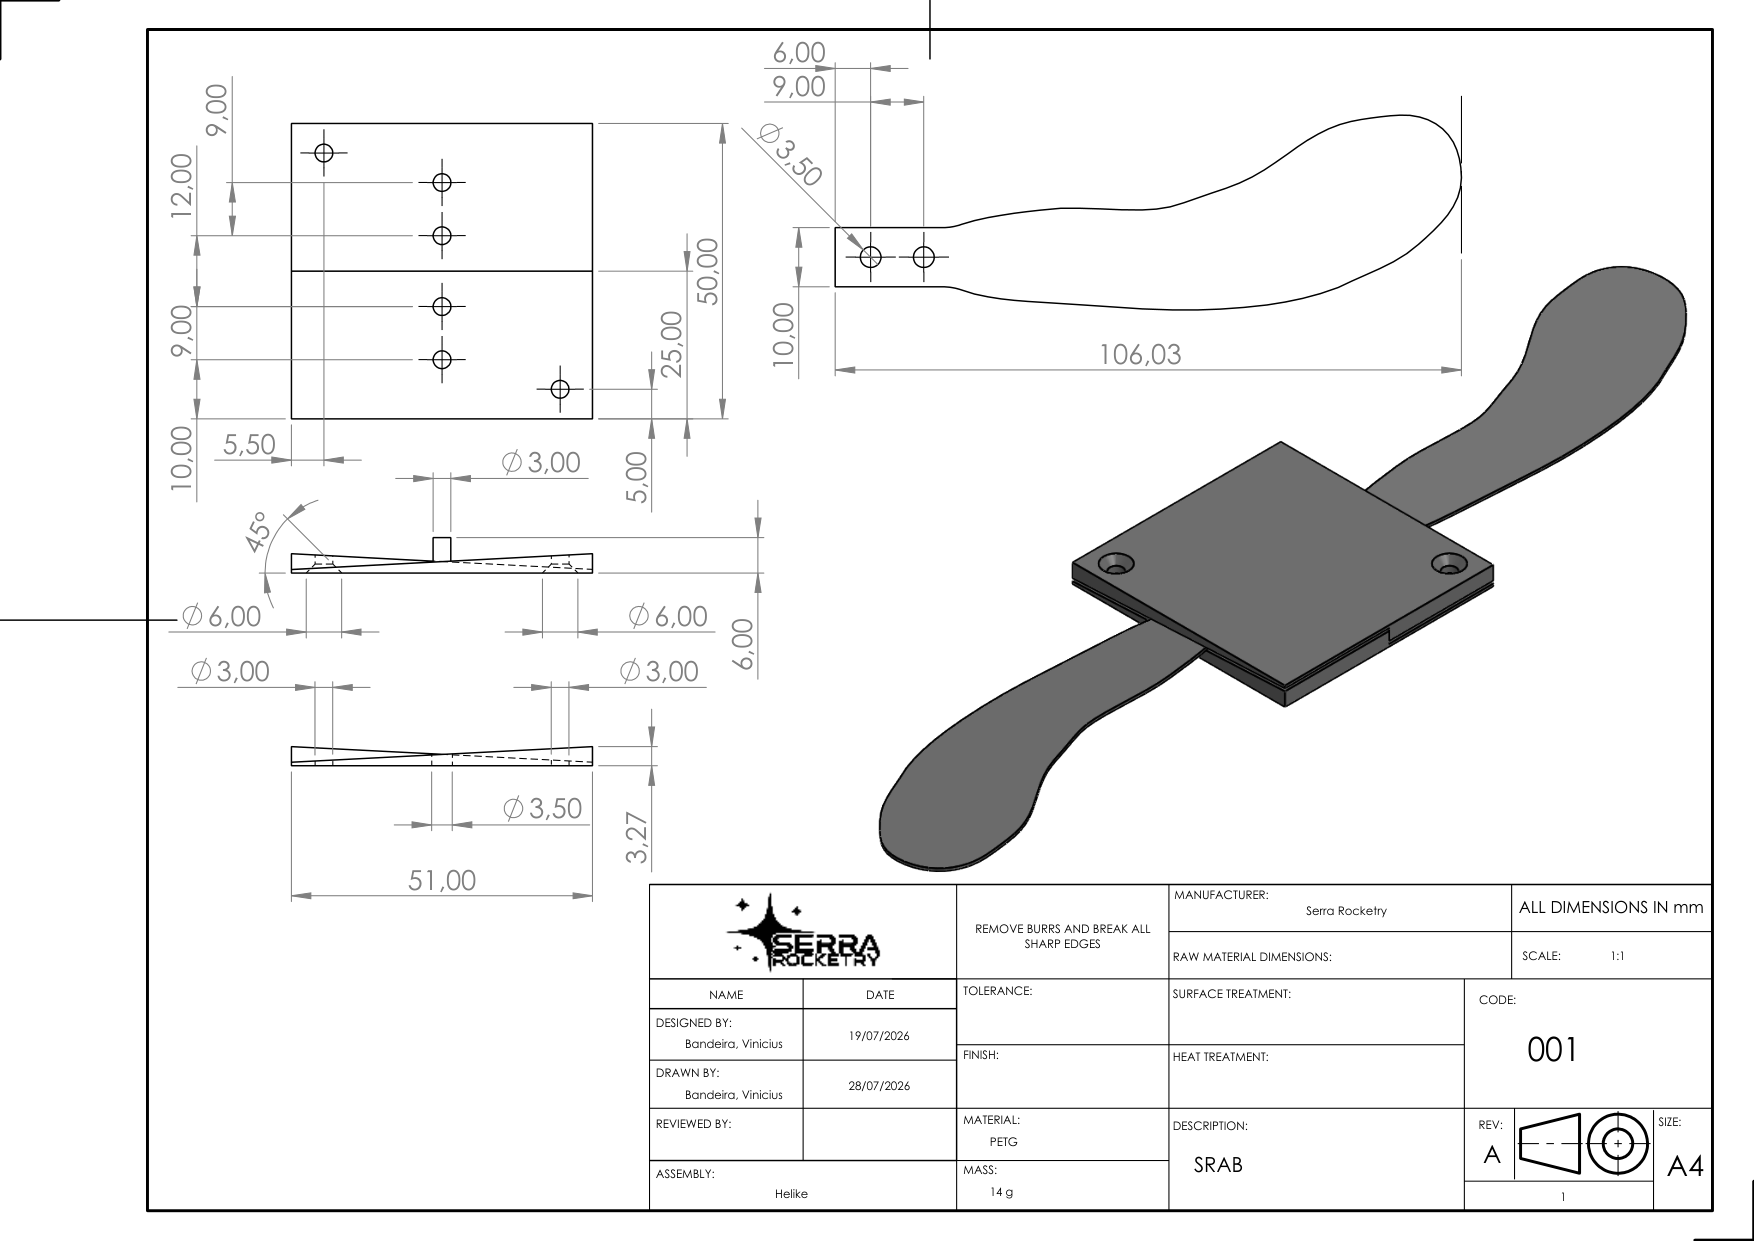
\includegraphics[width=0.8\textwidth]{figures/srab_only_assy_p1.png}
\caption{Technical drawing of the SRAB assembly: central 50$\times$50
mm hub and the two mirrored autorotative wings (PETG, total mass
14~g).}
\label{fig:srab-assembly}
\end{figure}

\begin{figure}[htbp]
\centering
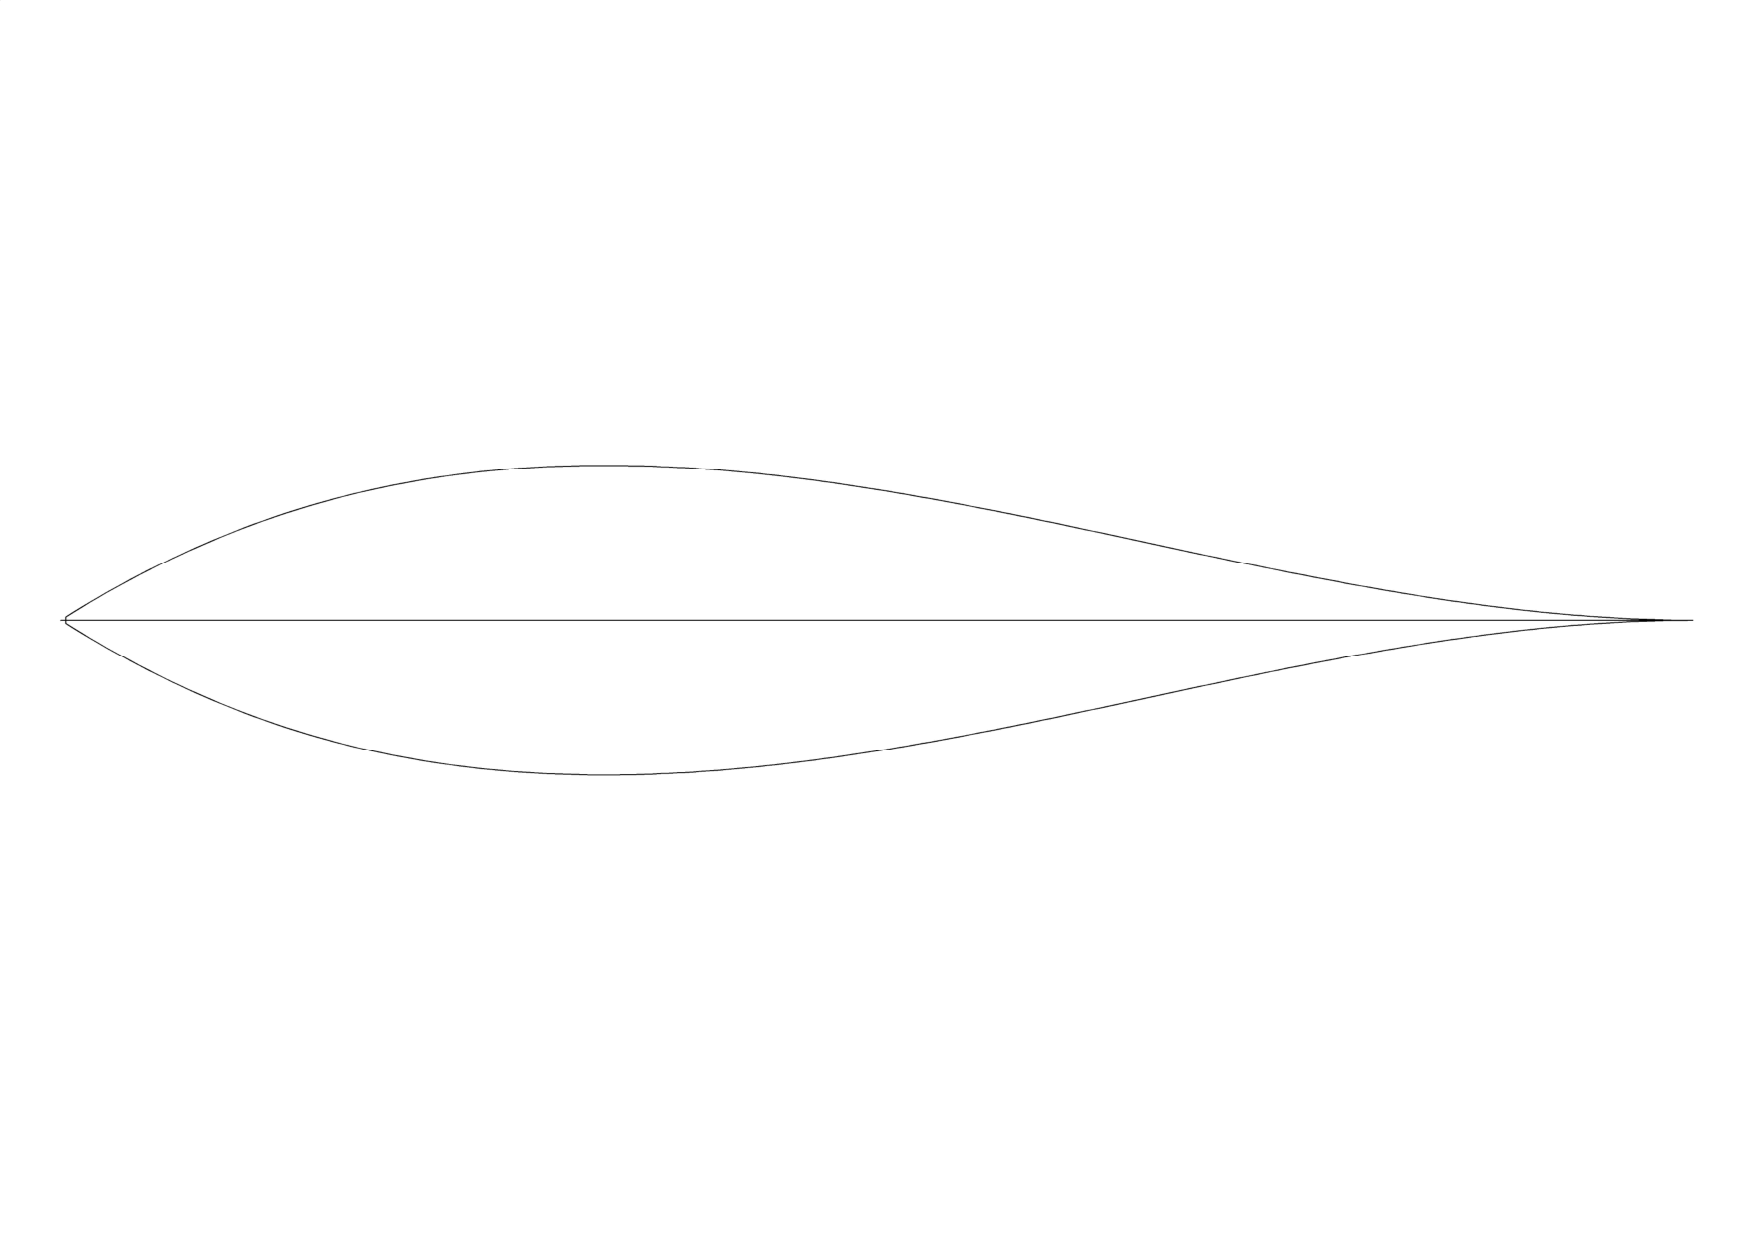
\includegraphics[width=0.9\textwidth]{figures/Asa1_dxf_p1.png}
\caption{2D contour drawing (DXF) of Asa1 wing geometry: 4-wing
configuration, base chord and tip dimensions marked. Used in the
first physical drop campaign (Test 1).}
\label{fig:asa1-dxf}
\end{figure}

\begin{figure}[htbp]
\centering
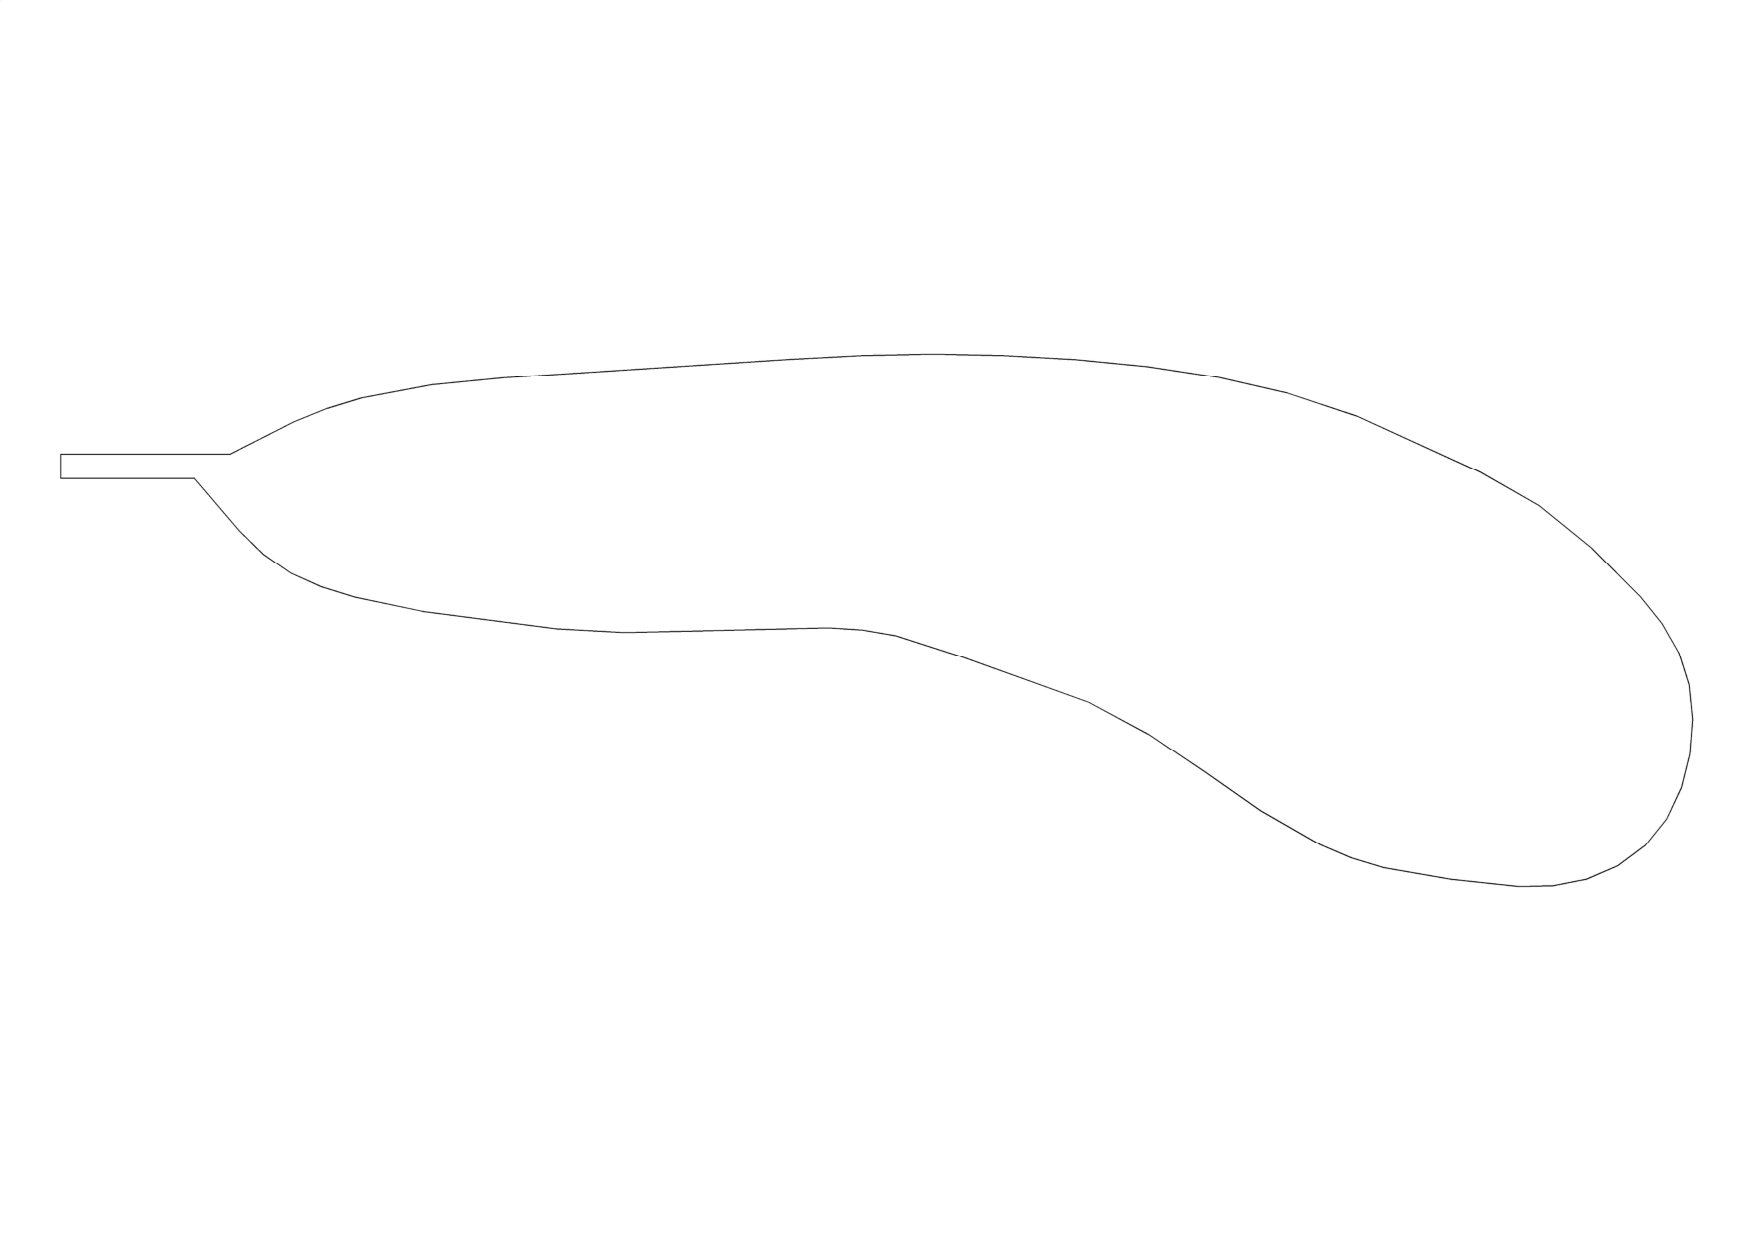
\includegraphics[width=0.9\textwidth]{figures/Asa2_dxf_p1.png}
\caption{2D contour drawing (DXF) of Asa2 wing geometry: 4-wing
configuration with increased area and realigned chord relative to
Asa1. Used in the second drop campaign (Test 2).}
\label{fig:asa2-dxf}
\end{figure}

\begin{figure}[htbp]
\centering
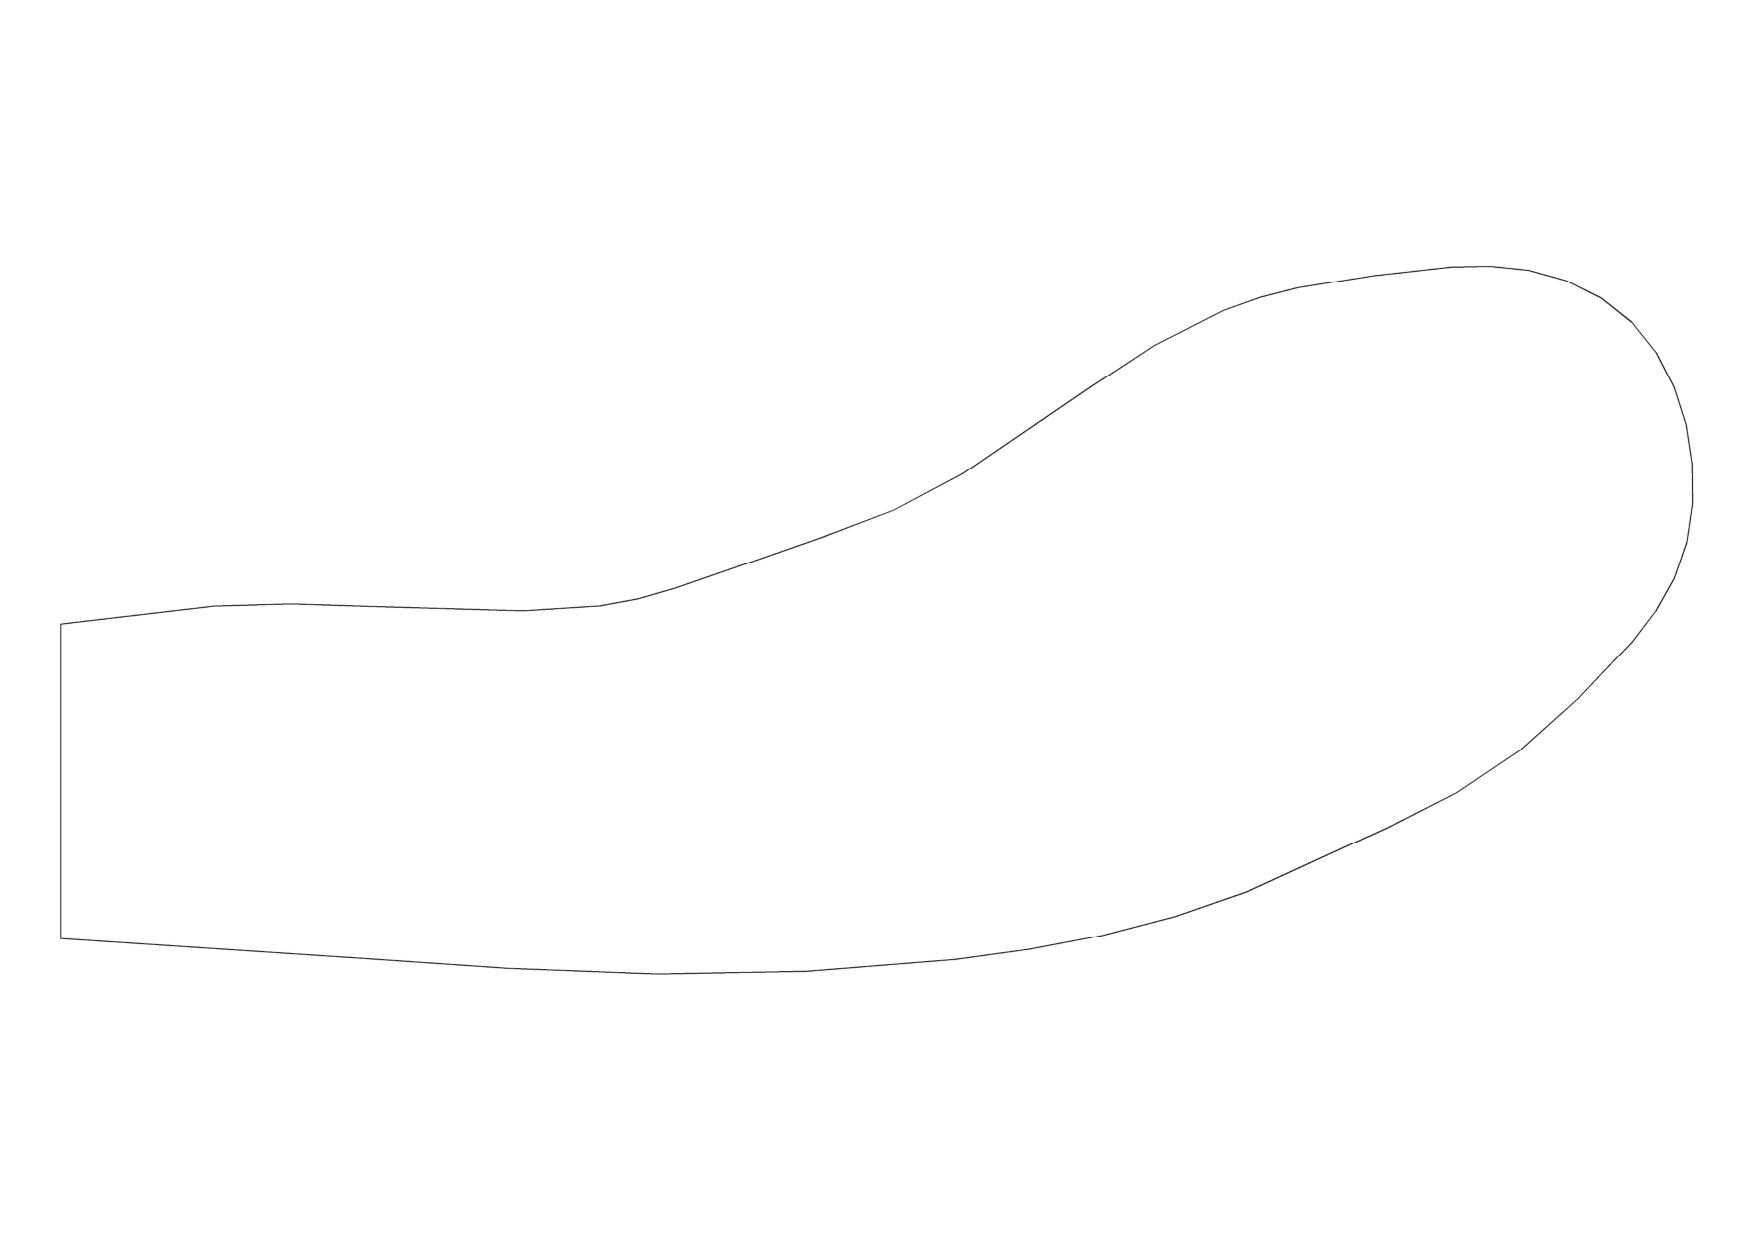
\includegraphics[width=0.9\textwidth]{figures/Asa3_dxf_p1.png}
\caption{2D contour drawing (DXF) of Asa3 wing geometry: 2-wing
mission-final configuration. Optimised radius 79.7~mm, chord and
pitch distribution for the target $V_F = 13.33$~m/s with FS 1.5.}
\label{fig:asa3-dxf}
\end{figure}

\subsection{Optional Appendices}

\subsubsection{SRAB Wing Geometry}

The wing geometries evolved through three design iterations, driven
by the simulation-to-field comparison loop described in Section 4:

\begin{itemize}
\item \textbf{Asa1} — 4 wings, first prototype: v$_{impact}$ =
  7.68~m/s, 306.8~rpm, 13.5$^{\circ}$.
\item \textbf{Asa2} — 4 wings, increased area and realignment:
  v$_{impact}$ = 8.04~m/s, 306.9~rpm, 24.4$^{\circ}$ — candidate
  configuration.
\item \textbf{Asa3} — 2 wings (mission final): reduced mass and
  complexity, $v \approx 13.33$~m/s terminal, within the LASC
  20~m/s limit with a 1.5 safety factor.
\end{itemize}

The 2D contour drawings (DXF) for each iteration are presented in
Fig.~\ref{fig:asa1-dxf}, Fig.~\ref{fig:asa2-dxf} and
Fig.~\ref{fig:asa3-dxf} above.

\subsubsection{Test Data}

% TODO: include CSV logs, telemetry plots, simulation-vs-field
% comparison plots, photos of Asa1/Asa2 prototypes and drop-test
% videos once the instrumentation campaign (Test 4, ~200 m) is
% complete.

\subsubsection{Computational Simulation}

The 4th-order autorotation model, calibrated parameters, simulation
scripts (RocketPy + SRAB extension) and the geometry heat-map are
maintained in the repository under \texttt{extras/wing-analysis/}.
The full-flight simulation (Dédalo + SRAB) is documented in the
notebook \texttt{01\_simulacao\_dedalo.ipynb}.
